\chapter{Literature Review}
\label{sec: Literature_review}
\section{Introduction}
    A rotary-wing aircraft is defined as a configuration in which during take-off and landing, the aircraft derives its lift force directly from an open airscrew, where an airscrew is any actuator disc that has air as its working fluid. These types of aircraft can hover and have Vertical Take-Off and Landing (VTOL) capabilities. Rotary aircraft's airscrews have been given the name of `Rotor' and are characterized by a low disc loading. Disc loading is defined as the average change in pressure across an airscrew. For a rotary aircraft, it is the ratio of the rotor disk area to the total weight of the aircraft (\cite{stepniewski1984rotary}). The most common example of a rotary aircraft is a helicopter. Over the years helicopters have evolved and have gone through many concepts. Tip thrust is one of these changes and will be the focus of this literature review. 

\section{Historical Development}
    One of the earliest concepts of a rotary aircraft can be traced back to Leonardo da Vinci, who came up with the idea of a flying machine based on the Archimedes screw. The Archimedes screw can be thought of as the precursor to the airscrews we have today. While Leonardo's design theoretically worked, it would have been too impractical to build a full-sized version, it did, however, inspire people to create vertical flight machines \citep{stepniewski1984rotary}.\\

    The second factor hindering the development of the helicopter was a lack of understanding of basic aerodynamics. Helicopters are inherently unstable and have a tendency to flip over when in forward flight, this was later discovered to be due to an asymmetrical distribution of lift across the rotor. This is caused by the fact that the lift produced is directly proportional to the incoming air speed squared (\(\text{lift}\;\alpha \text{ air speed}^2\)). When in forward flight one side of the rotor will be moving opposite to the direction of airflow and thus its relative air velocity is higher than the rotor moving in the same direction of the incoming air, one side having increased lift and the other a decreased lift, causing the asymmetry of the forces (\cite{anderson2010helicopters}). This was corrected using a swashplate as well as articulating the blade with flapping and feathering hinges.\\
    

    There were two main points that made the helicopter such a difficult task to accomplish. The first was a lack of an efficient power source. Before the combustion engine, the only power source was the steam engine, which would not produce enough thrust for its weight to make it a viable power source. Even with the combustion engine, it was only after World War I when they began using aluminum that a power-to-weight ratio became large enough to sustain flight. (\cite{stepniewski1984rotary})\\
    
    \begin{figure}[H]
        \centering
        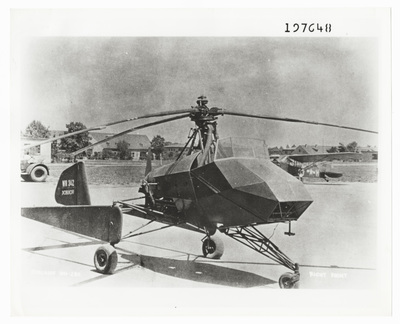
\includegraphics[width = 0.6\textwidth]{figs/WNF V4.jpg}
        \caption{WNF 342 V4 (\cite{Linenbaum_2020})}
        \label{fig:WNF_432_V4}
    \end{figure}

    The first concept of a tip-thrust helicopter can be traced back to the start of World War II, developed by a junior engineer at Wiener Neustädter Flugzeugwerke (WNF), Friedrich von Doblhoff. He proposed to place ramjets on the tip of the rotor and after a short-lived proof of concept managed to impress officials, Friedrich obtained the necessary funding for his first Jet-tipped aircraft. In total four prototypes were constructed, namely WNF 342 V1, V2, V3 and V4, with each design improving on the previous. WNF 342 V4, shown in  Figure~\ref{fig:WNF_432_V4}, used a supercharged engine modified as a compressor to provide air to the rotors and to provide thrust at the back with a pusher propeller. The final design noted that using the jet-tip was inefficient and was used for vertical take-off and landings, when in forward flight, the compressor was switched off, and it operated as an autogyro. Autogyros have freely rotating rotors that spin due to the force of incoming air, this in turn generates lift. The WNF 342 V4 
    design used a mechanism similar to a swashplate to control the cyclic pitch of the rotor and used the air pressure, along with torsional springs, to change the collective pitch (these concepts are further explained in Section~\ref{sec:Helicopter_Control}). The development of tip-thrust was stopped when the test facility was taken by the Allied forces, however, Mr. von Doblhoff would go on to work in America and work on compound helicopters, helicopters which are a hybrid between the rotary-wing and fixed-wing aircraft.  

\section{Helicopter Control} \label{sec:Helicopter_Control}
    Helicopter control relies on the pitch of each blade. The change in pitch causes a change in the angle of attack (AOA). The AOA is directly related to the lift coefficient through \[C_L = C_{L{_0}} +C_{L{_\alpha}} \cdot \alpha\] 
    \begin{minipage}{0.45\textwidth}
        \vspace*{-4mm}
        \begin{align*}
            \text{where} \quad
            &\,C_L \text{ is the coefficient of lift}\\
            &\, C_{L{_0}}\text{ is the offset}  \\
            &\,C_{L{_\alpha}}\text{ is the rate of change of \(C_L\) relative to the AOA}\\
            &\,\alpha \text{ is the angle of attack}\\
        \end{align*}
        \end{minipage}\\

    This is illustrated in Figure \ref{fig:Lift_Vs_AOA}(\cite{angleOfAttackFormula}). Thus increasing the angle of attack increases the lift coefficient, which increases the lift produced. This same concept can be applied to the drag coefficient (\(C_D\)) \\
    \begin{figure} [h]
        \centering
        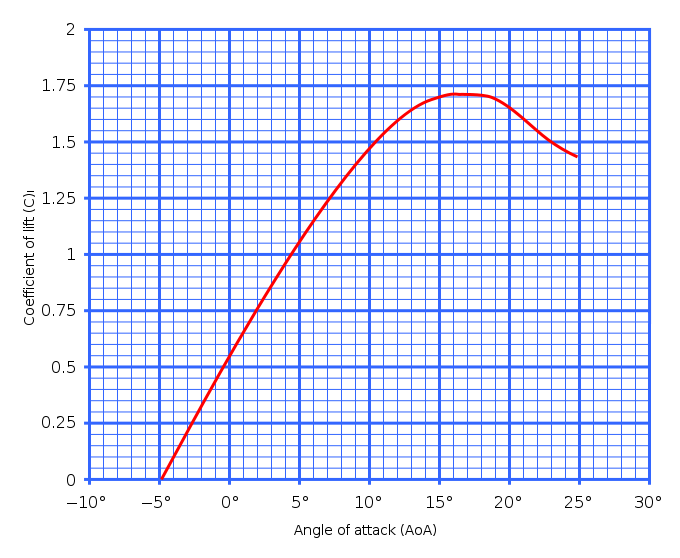
\includegraphics[width = 0.6\textwidth]{figs/Lift_Vs_AOA.png}
        \caption{Lift vs Angle of Attack (\cite{SKYbary})}
        \label{fig:Lift_Vs_AOA}
    \end{figure}

    Helicopters use collective and cyclic control during flight. The collective control adjusts the pitch of all the blades uniformly, this creates more or less lift overall, allowing the helicopter to rise or fall. The cyclic control varies the pitch depending on where the rotor is in its rotation. Traditional helicopters use swashplates to achieve this control.\\
    A swashplate consists of two plates connected with bearings. This allows the top plate to rotate and the bottom plate to remain fixed. The top plate is connected to the edge of each blade of the rotor by a pitch change arm. This allows control over the pitch by varying the height and angle of the swashplate as can be seen in Figure~\ref{fig:Swashplate} (\cite{anderson2010helicopters}.)
    \begin{figure}
        \centering
        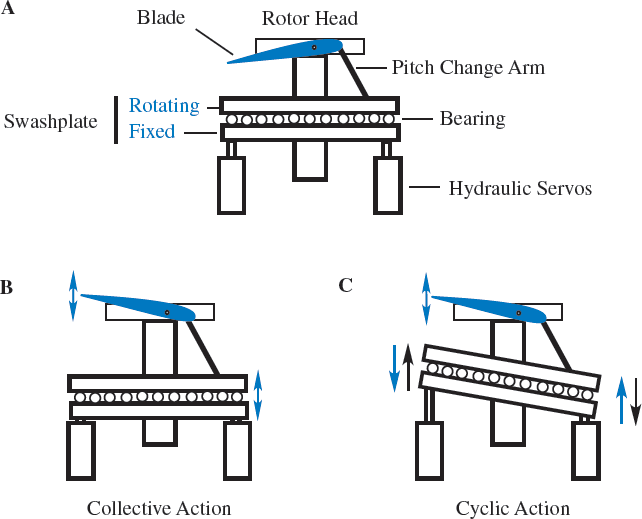
\includegraphics[width = 0.6\textwidth]{figs/Swashplate.png}
        \caption{Lift vs Angle of Attack (\cite{anderson2010helicopters})}
        \label{fig:Swashplate}
    \end{figure}

% The objectives of the project (in some cases the objectives of the report). If necessary describe limitations to the scope.

\section{Current State of the Art} \label{sec:Current_design}
    The concept of tip thrust is an unresearched area of development, however, there a still many applications of this technique, all of which have been applied in different ways. The commonality between all the designs is the method used for propulsion. While some methods make use of ramjets or liquid rockets attached to the tip, it was found during the student's investigation that many designs have been built to create thrust by ejecting an operating fluid out of a nozzle at the tip of the rotor blade. The temperature of the operating fluid splits into two subcategories, a cold-cycle and a hot-cycle. Cold-cycles use compressors and utilize compressed air as the operating fluid. Whereas a hot-cycle uses a gas generator that burns a mixture of compressed air and fuel, creating combustion of products (at temperatures greater than 700\(\degree\)C) which are used as the operating fluid \citep{elmahmodi2014propulsion}.\\
   
    NASA designed a very heavy-lift helicopter (VHLH) using the hot-cycle technique. This was designed as a solution to the weight constraints of shaft-drive helicopters. It was designed such that it could lift an XM-1 Main Battle Tank, which has a total weight of 60 tons, shown in Figure~\ref{fig:VHLH}. The helicopter has a fixed pitch rotor, which is used to generate lift, allowing for VTOL. To control the movement of this helicopter, as the pitch is fixed and cannot use conventional methods, a tail fan with a controllable pitch and controllable louvers, which direct the airflow, was installed at the back. Unfortunately, although the concept was very promising, it was never constructed \citep{head1981}.\\
    \begin{figure}[H]
        \centering
        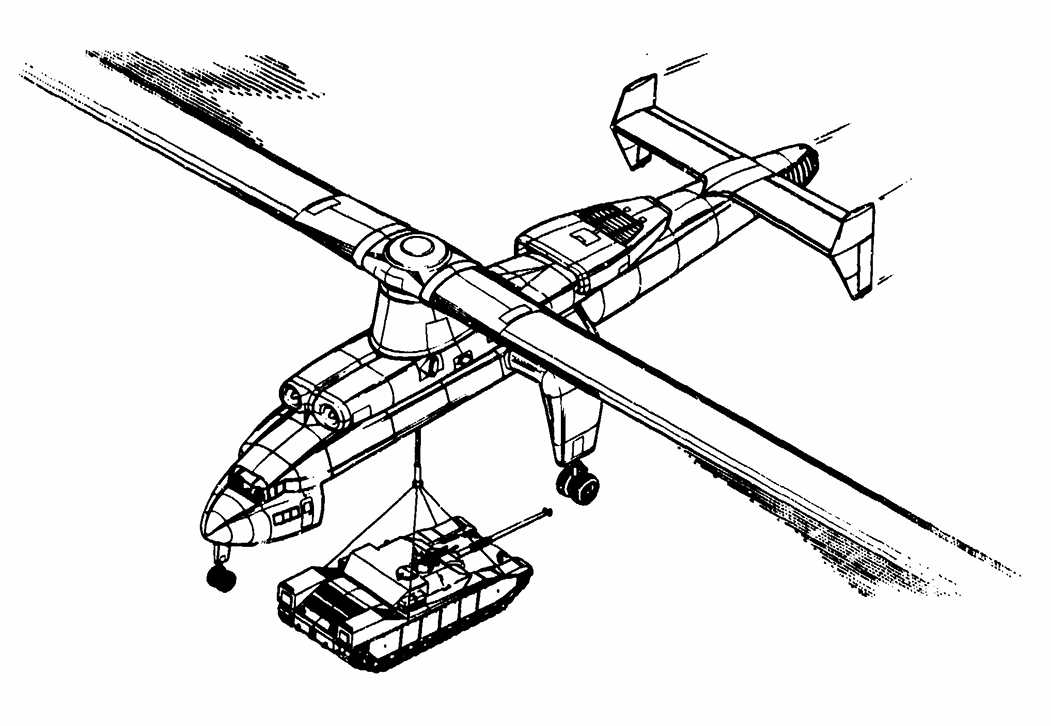
\includegraphics[width = 0.6 \textwidth]{figs/Heavy lift Helicopter.png}
        \caption{VHLF with a XM-1 Main Battle Tank payload}
        \label{fig:VHLH}
    \end{figure}

    The ATRO-X tip-jet helicopter is an example of a fully constructed jet-tipped helicopter that also makes use of a hot-cycle to provide propulsion. The gas generator is situated on top of the rotor and is connected to a flexible tube to the rotor. The operating fluid travels through the hollow rotors to the tips, where the fluid is expelled. This helicopter only has the main rotor, greatly simplifying the complexity of the helicopter, however, a study by \cite{KOLAREVIC2020112} showed that it was not as efficient as a conventional helicopter. This was partly due to the significant pressure drop of the operating fluid in the rotor channels. It was also stated that the efficiency could be increased by making the rotor larger, however this causes a larger pressure drop. To try to rectify this issue a study by \cite{elmahmodi2014propulsion} tried using the centrifugal force of the rotor as a radial compressor and proved the viability of this concept.\\

    The issues that each of the above concepts encountered will be used to guide all designs regarding the current proof of concept. The current designs have provided very useful insight into what concepts work and which have fundamental issues and should be avoided.

\section{Blade Element Theory}
This method is used to predict the performance of a blade, such as a rotor or a propeller as explained by \cite{blade_element_theory_2024}. The method achieves this by dividing the blade into multiple independent sections along the length of the blade as shown in Figure~\ref{fig: blade_segments}. A force balance is applied to each 2D section to obtain the lift and drag as well as the torque and thrust produced over the section. These values can be summed to predict the total thrust and torque produced by the rotor. \\
As this theory considers the 2D segments, it does not take 3D effects into account, such as flow velocities induced on the blade by the shed tip vortex or the radial component created by the angular acceleration due to the rotation of the rotor. This results in the model overpredicting the thrust produced and underpredicting the torque, resulting in a theoretical efficiency that is between 5\% to 10\% larger than the measured efficiency. One of the flow assumptions made is that the flow on the blade is not stalled, which needs to be kept in mind when designing the system.
\begin{figure}
    \centering
    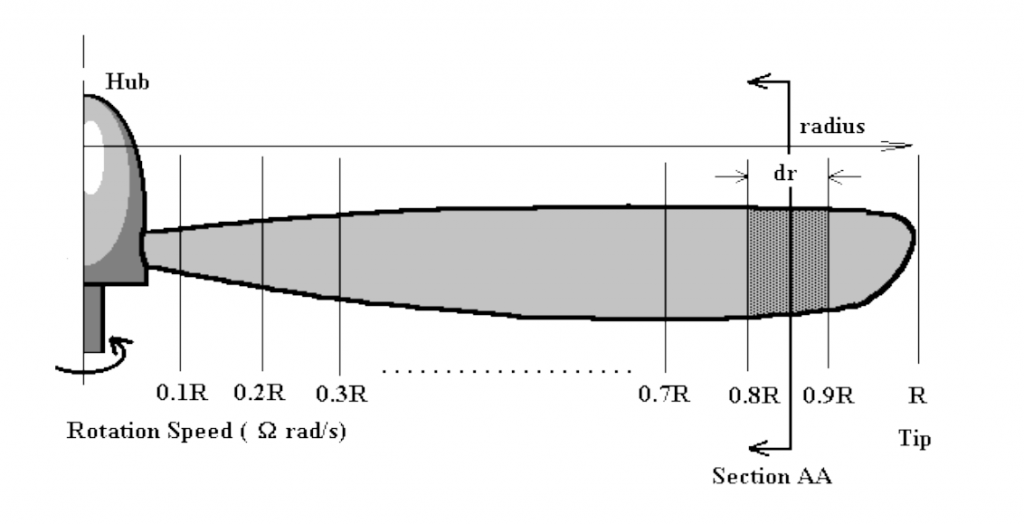
\includegraphics[width =0.8\textwidth]{figs/Blade_Element.png}
    \caption[Segmented blade]{Diagram showing the blade split into segments \citep{blade_element_theory_2024}}
    \label{fig: blade_segments}
\end{figure}

As shown in Figure~\ref{fig: blade_segments}, the blade can be subdivided to make multiple discrete sections. For this analysis, only the axial and angular components, V\(_0\)  and V\(_2\) respectively, as labeled in Figure~\ref{fig: blade_forces}, of the velocity will be used. The induced flow is assumed to be negligible. V\(_1\) is the summation of these two velocities. 

\begin{figure}[h]
    \centering
    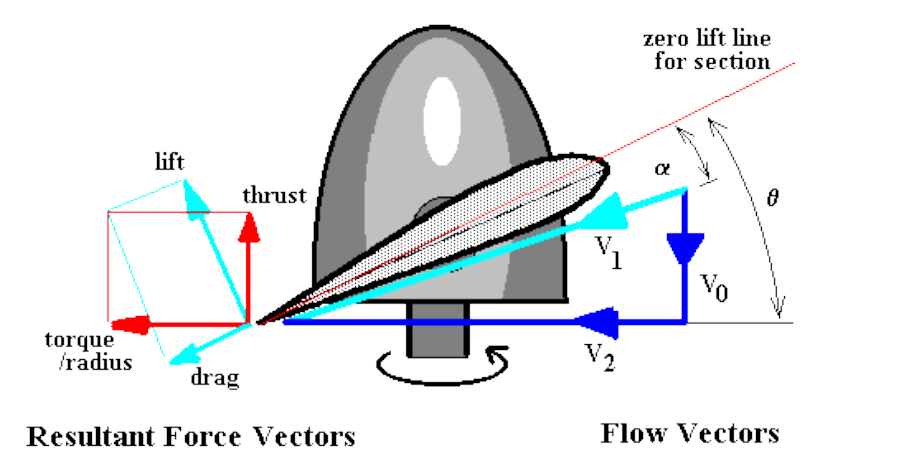
\includegraphics[width =0.8\textwidth]{figs/Blade_Forces.png}
    \caption[Forces acting on the 2D section AA]{Forces acting on the 2D section A-A of Figure~\ref{fig: blade_segments} \citep{blade_element_theory_2024}}
    \label{fig: blade_forces}
\end{figure}
Theta, \(\theta\),  shown in Figure~\ref{fig: blade_forces} is the geometric pitch of the blade. The angle created between the flow velocity vector (V\(_1\)) and \(\theta\) creates the angle of attack~(\(\alpha\)). The lift and drag components are normal and parallel, respectively,  to the blade disk and can be calculated, using Eq. \ref{eq: lift_equation} and Eq. \ref{eq: drag_equation}, to find the thrust and torque of the blade. 
\begin{align}
    \Delta L &= C_L \frac{1}{2} \rho V_1^2 c.dR \label{eq: lift_equation}\\
    \Delta D &= C_D \frac{1}{2} \rho V_1^2 c.dR \label{eq: drag_equation}
\end{align} 
\begin{minipage}{0.45\textwidth}
\vspace*{-8mm}
\begin{align*}
    \text{where} \quad
    &C_L \text{ and } C_D \text{ are for a given } \alpha &\notag \\
    &\rho \text{ is the air density} \notag \\
    &c \text{ is the blade chord} \notag
\end{align*}
\end{minipage}
\\

The difference in angle between thrust and lift can be defined as \[\varphi = \theta - \alpha\] and thus thrust and torque can be found as 
\begin{align}
    \Delta T &= \Delta L\cos(\varphi) - \Delta D\sin(\varphi)  \label{eq: thrust}\\
    \frac{\Delta Q}{R} &= \Delta D\cos(\varphi) + \Delta L\sin(\varphi)  \label{eq: torque}
\end{align}
Combining Eq. \ref{eq: lift_equation} and Eq. \ref{eq: drag_equation} with Eq. \ref{eq: thrust} and Eq. \ref{eq: torque} yields
\begin{align}
    \Delta T &=  \frac{1}{2} \rho V_1^2 c (C_L\cos(\varphi) - C_D\sin(\varphi)) B. dR\\
    \Delta D &=  \frac{1}{2} \rho V_1^2 c (C_D\cos(\varphi) + C_L\sin(\varphi) )B.R.dR
\end{align}
\begin{minipage}{0.45\textwidth}
    \vspace*{-8mm}
    \begin{align*}
        \text{where} \quad
        &B  \text{ is the number of blades} 
    \end{align*}
    \end{minipage}

    \section{Momentum Theory}
        \begin{figure}[h]
            \centering
            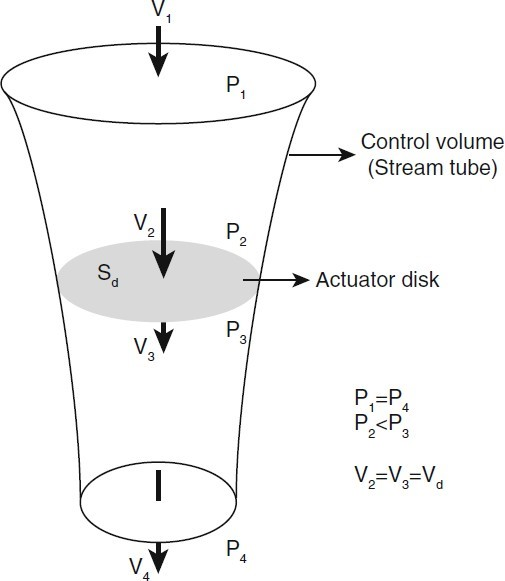
\includegraphics[width =0.6\textwidth]{figs/Literature Review/Momentum_theory.png}
            \caption{Momentum theory airstream velocities}
            \label{fig: mometum_theory}
        \end{figure}
        Momentum theory simplifies the rotor of the helicopter's rotor by viewing it as a disc that air flows through and energy is imparted on it by the rotor as stated in  \cite{AflredAerodynamicsOfHelicopters}. As shown in Figure~\ref{fig: mometum_theory}, velocity increases from \(V_0\) to \(V_3\), and it is assumed that the air follows the streamlines, indicated in Figure~\ref{fig: mometum_theory}. The naming convention for the velocities apply only to this section, throughout the report \(V_0,V_1,V_2\) will be as defined in Figure~\ref{fig: blade_forces}. From the mass conservation equation, we know that the \(\dot{m} = \rho S_d V\), through the rotor, thus \(\rho_1 S_1 V_1 = \rho_2 S_2 V_2 = \rho_3 S_3 V_3 =  \rho_4 S_4 V_4 = \text{constant} \), therefore the thrust can be given by
        \begin{align}
            T = \rho S_2 V_1(V_4-V_2) \label{eq: thrust_1}
        \end{align}
         Thrust can also be found as the difference of pressure, \(T=S_2(P_2-P_3)\). Applying Bernoulli's equation which states that the static and dynamic pressure at \(P_1\) be equal to that at \(P_2\), similarly for  \(P_3 \text{ and } P_4\), as \(V_2=V_3\).
        \begin{align*}
           P_1 +\frac{1}{2}\rho V_1^2 &= P_2 +\frac{1}{2}\rho V_2^2 \\
           P_3 +\frac{1}{2}\rho V_3^2 &= P_4 +\frac{1}{2}\rho V_4^2 
        \end{align*}
        These can be rearranged to give
        \begin{align}
            P_3 - P_2 &= \frac{1}{2}\rho(V_4^2 - V_1^2) \notag\\
            \Rightarrow  T &= \frac{1}{2}\rho S(V_4^2 - V_1^2) \label{eq: thrust_2}
        \end{align}
        Making Eq.~\ref*{eq: thrust_1} equal to Eq.~\ref*{eq: thrust_2} we get
        \begin{align*}
            \rho S_2 V_0(V_4-V_1) &=\frac{1}{2}\rho S(V_4^2 - V_1^2)
        \end{align*} 
        which simplifies to
        \begin{align}
            \frac{1}{2}(V_4 + V_1) = V_2 = V_3
        \end{align}

        \section{Gyroscopic Procession}
            This is a phenomenon due to the conservation of angular momentum. It occurs when a force is applied to a rotating object. This force changes the direction of the angular momentum vector. Results in the effects of the applied torque are felt 90\(^circ\) from where the force was applied, as seen in Figure~\ref{fig: gyroscope_procession}. This will cause a helicopter pilot to produce more thrust, by increasing the pitch, at a 90\(^\circ\) offset from the direction the pilot wishes to travel in \citep{gyro}.
        \begin{figure}[H]
        \centering
        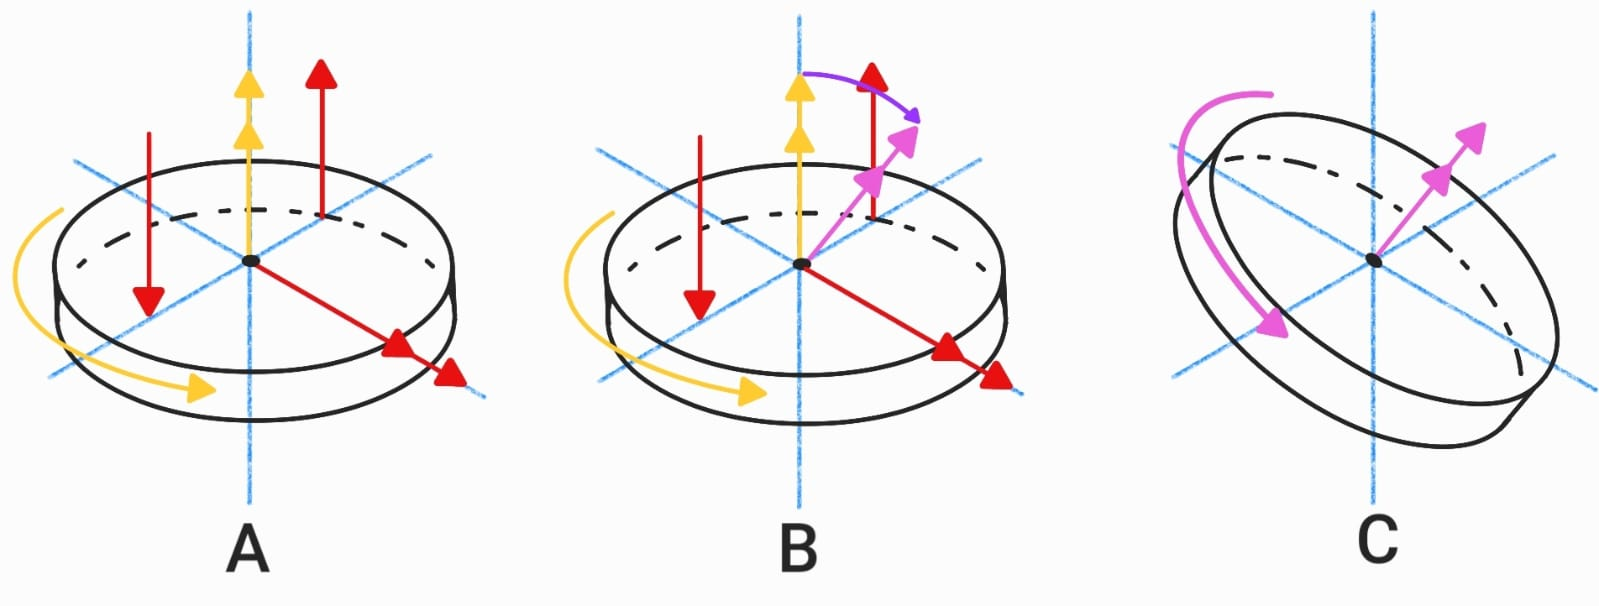
\includegraphics[width =\textwidth]{figs/Literature Review/Gyroscopic procession.jpg}
        \caption{Gyroscopic procession}
        \label{fig: gyroscope_procession}
\end{figure}